\chapter{The Baryon Sector: Confinement and Fractional Quarks}
\label{ch:baryons}

\begin{objectivebox}
\begin{itemize}
    \item Understand the $6^3_2$ Borromean linkage topology that structurally enforces quark confinement.
    \item Evaluate the precise derivation of the proton-to-electron mass ratio ($1836.15$) from the non-linear Faddeev-Skyrme energy functional.
    \item Deconstruct the fundamental forces by unifying the Strong Force and Macroscopic Gravity algebraically through the Hierarchy Bridge.
\end{itemize}
\end{objectivebox}

\textbf{A-034 nuclear-scale instance (canonical 2026-05-15 evening):} the
proton (and DT fusion at the nucleon-binding scale) is an explicit row in
the A-034 catalog (Universal Saturation-Kernel Strain-Snap Mechanism). Per
Grant 2026-05-15: \emph{``the bulk response of the lattice to strain is
universal.''} The Faddeev-Skyrme energy functional and Axiom 4 gradient
saturation invocations throughout this chapter all reduce to the same
universal kernel $S(A) = \sqrt{1 - A^2}$ that governs atomic dielectric
breakdown, BCS superconductivity, BH ring-down, and cosmic K4 crystallization
at appropriate scales. Specifically, the nuclear topology snap (DT fusion
$\to$ neutron ejection + $^4$He alpha collapse) is the nuclear-scale
manifestation: when the inter-nucleon strain crosses the bond-yield
threshold, the topology reorganizes catastrophically, releasing 14.1 MeV
in the neutron channel. See Vol 3 Ch 4 \S\ref{sec:tki_strain_snap}
+ Backmatter Ch~\ref{app:universal_saturation_kernel} for the full 26-instance
catalog.

The baryon sector introduces a fundamentally different class of topology from the leptons. While leptons are modeled as single, isolated standing waves (Hopfions), baryons are defined by the mutual entanglement of multiple distinct loops of electromagnetic momentum flux ($\mathbf{A}$).

\section{Borromean Confinement: Deriving the Strong Force}
The proton is modeled not as a bound state of independent point particles, but as a rigid \textbf{Borromean Linkage} of three continuous electromagnetic phase-flux loops ($6^3_2$) resonant within the discrete LC network. The Borromean rings consist of three LC standing waves interlinked such that no two individual loops are linked directly, but the three together form an inseparable resonant triad. This optical geometry intrinsically enforces \textbf{Quark Confinement}.

\begin{figure}[h]
    \centering
    
\includegraphics[width=0.85\textwidth]{borromean_proton_3d.png}
    % [2026-06-15 KB-reconciliation LF-03 driver-honesty-twin (vol_2) -- prior wording preserved per Rule 12]: read "The central toroidal void derives the $938.27 \text{ MeV}$ rest mass". SUPERSEDED: this figure is a 3D parametric visualisation only -- it does NOT compute the proton mass (per src/scripts/vol_2_subatomic/simulate_borromean_baryon.py, language softened 2026-05-17). The mass is the Faddeev-Skyrme eigenvalue (the 1-residual result at :217 + \kbleaf{ave-kb/vol2/particle-physics/ch02-baryon-sector/self-consistent-mass-oscillator.md} :64), not derived by this plot. No value change.
    \caption{\textbf{The $6^3_2$ Borromean Topology of the Proton.} (Simulation Output --- 3D visualisation only). Three interlocked phase loops geometrically locked into the irreducible $6^3_2$ Borromean linkage. The central toroidal void is the geometric structure whose Faddeev--Skyrme energy eigenvalue yields the $938.27 \text{ MeV}$ rest mass (a 1-residual result derived in this chapter, \emph{not} computed by this 3D plot), framing Quark Confinement as spatial knot frustration rather than a phenomenological bound state.}
    \label{fig:borromean_proton_3d}
\end{figure}

\textbf{Resolving the Scale Paradox:} A challenge in discrete models is reconciling the empirical $0.84 \text{ fm}$ charge radius of the proton with a fundamental lattice pitch of $\ell_{node} \approx 386 \text{ fm}$. The AVE framework resolves this via solid-state scattering theory. The $0.84 \text{ fm}$ measurement is not the bounding box of the geometric loops. The $6^3_2$ Borromean knot spans multiple fundamental nodes. However, the orthogonal intersections of these three flux tubes generate localised tensor strain gradients ($\partial_\mu \mathbf{n} \times \partial_\nu \mathbf{n}$). In deep inelastic scattering experiments, high-energy probes scatter off the RMS average of these internal geometric strain gradients. The $0.84 \text{ fm}$ radius corresponds to the Root-Mean-Square (RMS) effective scattering cross-section of the topological core gradients, permitting sub-fermi empirical signatures to emerge from a $386 \text{ fm}$ structural array without violating the fundamental spatial cutoff limit (Axiom 1).

\subsection{The Topological Scaling Ansatz}

% 🔴 Rule-12 2026-06-21 INVARIANT-N1 𝓜_A→prose retirement: the retired $\mathcal{M}_{A}$ glyph (Amorphous-substrate symbol, retired 2026-06-18 per INVARIANT-N1 — the "A" carried the closed geometry-leak "amorphous") is replaced in this chapter by substrate-native prose ("substrate lattice" here; "chiral LC network" at the He-4 core-gradient site below). Physics + every number unchanged.
Because the vacuum operates as a discrete LC network, extreme spatial separation causes the phase-flux lines connecting the Borromean loops to collimate tightly into a 1D cylindrical tube rather than spreading out isotropically. The baseline 1D continuous electromagnetic string tension of the unperturbed substrate lattice evaluates to $T_{EM}=m_{e}c^{2}/\ell_{node}\approx0.212\text{ N}$. Standard Lattice QCD measures the empirical macroscopic strong force string tension at exactly $\approx 1\text{ GeV/fm}$ ($\approx 160,200\text{ N}$). 

While the 3D non-linear orthogonal tensor trace ($\mathcal{I}_{tensor}$) of the saturated $6_2^3$ Borromean linkage requires continuous elastodynamic simulation to solve analytically, the physical boundary conditions dictate a steady-state scaling relationship. The following \textbf{Topological Scaling Ansatz} is proposed: because the proton is a saturated Borromean linkage, the baseline tension bounding the quarks is geometrically amplified by three structural multipliers: the number of topological loops (3), the relative inductive resonance mass ratio ($m_p/m_e$), and the dielectric saturation boundary ($\alpha^{-1}$). Using the empirical CODATA proton mass ratio ($\approx 1836.15 \ m_e$)~\cite{codata2018} as a preview (the eigenvalue is derived in Section~\ref{sec:thermal_softening}):

\begin{resultbox}{Topological Scaling Ansatz}
\begin{equation}
    F_{confinement} \approx 3\left(\frac{m_p}{m_e}\right)\alpha^{-1}T_{EM} = 3(1836.15)(137.036)(0.212\text{ N}) \approx \mathbf{160,024\text{ N}}
\end{equation}
\end{resultbox}
    
Using the geometrically derived eigenvalue ($\approx 1836\ m_e$, Section~\ref{sec:thermal_softening}) instead yields $\approx 160{,}037\text{ N}$, or $\approx 0.999\text{ GeV/fm}$. Pending full dynamic computational evaluation of the $\mathbb{Z}_3$ tensor trace, this phenomenological ansatz bounds the macroscopic strong force at the expected $\approx 1\text{ GeV/fm}$ target using the framework's native theoretical outputs.

\section{The Proton Mass: The Dynamic Tensor Deficit}

The empirical mass ratio $m_p/m_e \approx 1836.15$ emerges dynamically as the exact eigenvalue of non-linear inductive resonance. The steady-state proton mass is evaluated by mapping it to the Faddeev-Skyrme non-linear Hamiltonian. Bounded by the strict squared dielectric limit ($n=2$) established in Axiom 4 to match standard QED optics, the static energy functional evaluates as:
\begin{resultbox}{Saturated Faddeev-Skyrme Proton Energy}
\begin{equation}
E_{proton} = \min_{n} \int d^3x \left[ \frac{1}{2}(\partial_\mu n)^2 + \frac{1}{4}\kappa_{FS}^2 \frac{(\partial_\mu n \times \partial_\nu n)^2}{\sqrt{1 - (\Delta\phi / \alpha)^2}} \right]
\end{equation}
\end{resultbox}

\subsection{The Faddeev-Skyrme Coupling Constant ($\kappa_{FS}$)}

The quartic Skyrme stabilization term requires a dimensionless coupling constant $\kappa_{FS}$ that sets the relative strength of the fourth-order repulsive gradient against the second-order attractive gradient. In the AVE framework, this coupling is not a free parameter but is derived directly from the packing fraction:
\begin{resultbox}{Faddeev-Skyrme Coupling Constant}
\begin{equation}
\kappa_{FS}^{(cold)} = \frac{p_c}{\alpha} = \frac{8\pi\alpha}{\alpha} = \mathbf{8\pi}
\end{equation}
\end{resultbox}

This is a pure geometric constant: the solid-angle normalisation ($4\pi$) of the spherical energy integral, doubled by the two orthogonal principal strain axes of the LC network that jointly stabilize the defect against Derrick-type collapse.

\subsection{Thermal Lattice Softening ($\delta_{th}$)}
\label{sec:thermal_softening}

The cold ($T=0$) Faddeev-Skyrme solver with $\kappa_{FS} = 8\pi$ evaluates the 1D scalar trace to $\mathcal{I}_{scalar}^{(cold)} \approx 1185\,m_e$, yielding a proton ratio of $\approx 1872$ (approximately $2\%$ above the empirical value). This systematic overestimate arises because the solver computes the ideal zero-temperature ground state, whereas the physical proton exists as a localized thermal hotspot within the LC network at an effective core temperature of $T_{core} \sim m_p c^2/k_B \approx 10^{13}\text{ K}$.

The baseline RMS thermal noise of the vacuum (``quantum foam'') partially averages out the sharp gradient tensor $(\partial_\mu \mathbf{n} \times \partial_\nu \mathbf{n})^2$, effectively softening the quartic Skyrme repulsion.  Additionally, the Faddeev-Skyrme energy functional includes Axiom~4 gradient saturation $S(|\partial_r\phi|,\,\pi/\ell_{node})$ inside the integrand, preventing the solver from resolving sub-lattice gradients.  The thermally corrected coupling is:
\begin{resultbox}{Thermal Lattice Softening}
\begin{equation}
\kappa_{FS} = \kappa_{FS}^{(cold)} \left(1 - \delta_{th}\right) = 8\pi\left(1 - \frac{1}{14\pi^2}\right)
\end{equation}
\end{resultbox}

where the residual thermal correction factor $\delta_{th} = 1/(14\pi^2)$ captures the RMS noise averaging that remains after the gradient saturation is applied:
\begin{enumerate}
    \item $\nu_{vac} = 2/7$ --- the Poisson ratio of the chiral LC lattice, which sets the anharmonic Gr{\"u}neisen parameter governing the coupling between thermal fluctuations and elastic stiffness.
    \item $\kappa_{cold} = 8\pi$ --- the Faddeev-Skyrme coupling (Skyrme stiffness).
    \item $2/\pi$ --- the mean-to-peak ratio of rectified sinusoidal thermal noise. With the peak gradient already saturated by Axiom~4, the residual averaging acts on only the mean component.
\end{enumerate}

The product evaluates to $\delta_{th} = \frac{\nu_{vac}}{\kappa_{cold}} \times \frac{2}{\pi} = \frac{2/7}{8\pi} \times \frac{2}{\pi} = \frac{1}{14\pi^2} \approx 0.00721$. Together with the gradient saturation inside the energy functional, this produces proton mass agreement to better than $0.1\%$ and covers the baryon ladder through crossing number $c = 15$ with maximum error $\sim 2.4\%$. \emph{Read ``covers'' as consistency, not ensemble-validation} (scope correction 2026-06-19, see the section-level note below the prediction table): the load-bearing positive is the single proton hit + the curved ladder FORM, not a six-state forward-validation.

\begin{figure}[h]
    \centering
    
\includegraphics[width=1.0\textwidth]{thermal_skyrmion_comparison.png}
    \caption{Cold ($\kappa = 8\pi$) vs.\ thermally corrected ($\kappa_{eff} = 8\pi(1-\delta_{th})$) Skyrmion profiles. Left: the hedgehog profile $f(r)$ broadens slightly under thermal softening. Right: the radial energy integrand $r^2\mathcal{E}(r)$ decreases by approximately 2\%, shifting $\mathcal{I}_{scalar}$ from $\sim 1185\,m_e$ to $\sim 1160\,m_e$.}
    \label{fig:thermal_skyrmion}
\end{figure}

\subsection{The 3D Orthogonal Tensor Trace ($\mathcal{I}_{tensor}$)}
While the 1D scalar radial projection of the saturated topological Hamiltonian assumes spherical symmetry, the Proton is a $6^3_2$ Borromean linkage possessing $\mathbb{Z}_3$ discrete permutation symmetry. Because the three constituent flux tubes are mutually orthogonal, they cross over each other within the saturated structural core. In an LC resonant network, intersecting confined electromagnetic flux lines generate anisotropic \textit{Transverse Polarization Strain}. 

The total RMS energy integral is decomposed into two distinct geometric trace components: the continuous spherical scalar trace ($\mathcal{I}_{scalar}$), and the discrete orthogonal intersection trace ($\mathcal{I}_{tensor}$):
\begin{resultbox}{Proton Mass Geometric Decomposition}
\begin{equation}
m_p c^2 = \mathcal{I}_{scalar} \text{ (1D)} + \mathcal{I}_{tensor} \text{ (3D Orthogonal Crossings)}
\end{equation}
\end{resultbox}

The thermally corrected 1D solver, with Axiom~4 gradient saturation applied inside the integrand, evaluates the scalar component to $\mathcal{I}_{scalar} \approx 1162\,m_e$. The remaining mass generation is contained within the orthogonal topological interference vectors of the intersecting flux loops.

\subsection{Computational Proof: Skew-Lines and The Toroidal Halo}
To analytically resolve the 3D orthogonal tensor trace ($\mathcal{I}_{tensor}$), the non-linear geometric frustration of the proton's spatial topology. The $6^3_2$ Borromean linkage is mathematically defined by exactly six orthogonal topological crossings.

By Axiom 1, the Full-Width at Half-Maximum (FWHM) of a fundamental flux tube is $1.0 l_{node}$. Furthermore, the hard-sphere exclusion principle dictates that orthogonal tubes cannot collide at a distance closer than $1.0 l_{node}$. To satisfy this constraint during 3D PDE integration, the flux tubes are modelled as \textbf{Skew Lines}, offset from one another by $1.0 l_{node}$ along their orthogonal axis.

When evaluated continuously across the discrete grid, this skew-line topology reveals a notable geometric symmetry:
\begin{enumerate}
    \item At the exact 3D geometric midpoint between the two separated tubes, the Gaussian strain fields of the individual tubes evaluate to exactly $0.5$. 
    \item Their scalar sum peaks at $0.5 + 0.5 = \mathbf{1.0}$. The overlapping geometry reaches the Axiom 4 dielectric saturation limit without requiring arbitrary scaling coefficients.
    \item Because the tubes are strictly orthogonal and geometrically symmetric, all transverse spatial gradients ($\partial_\mu n$) evaluate identically to zero at the exact geometric center.
\end{enumerate}

Consequently, the cross-product vector ($\nabla V_1 \times \nabla V_2$) evaluates to zero. The topological metric bypasses the $0/0$ L'Hôpital singularity. The mass generation cannot collapse into a point singularity; instead, the localised spatial metric is pushed outward, forming a stable, saturated 3D \textbf{Toroidal Halo} of tensor shear.

\subsection{The Self-Consistent Mass Oscillator (The Structural Eigenvalue)}
To convert the orthogonal tensor trace into a closed-form mass prediction, one must first analytically resolve the total saturated volume $\mathcal{V}_{total}$ of the toroidal halo formed by the six orthogonal crossings.

\textbf{Counting the saturated crossings.} The $6^3_2$ Borromean linkage consists of three mutually orthogonal loops, each pair of which crosses exactly twice. The total number of pairwise orthogonal crossings is therefore $\binom{3}{2} \times 2 = 6$. By the $\mathbb{Z}_3$ permutation symmetry of the linkage, all six crossings are geometrically equivalent under discrete rotation.

\textbf{The saturation threshold (under a Gaussian flux-tube ansatz).} The critical advance in evaluating $\mathcal{V}_{total}$ is determining the density threshold at which the combined flux-tube field becomes topologically locked. This threshold is derived from the mutual inductance coupling between the orthogonal LC flux loops at their crossings, conditional on the radial profile of the flux tube.

\paragraph{Profile ansatz (open derivation gap).} The $\sigma$ derivation below assumes a \textbf{Gaussian flux-tube radial profile} with FWHM $= \ell_{node}$. Axiom 1 fixes the FWHM (Nyquist content: the smallest unambiguously-resolvable transverse feature is one lattice pitch), but it does not specify the functional form. The Gaussian is an \emph{ansatz} for tractability; other LC-soliton profiles (sech$^2$ kink, Bessel $J_0$ waveguide fundamental, the algebraic Axiom~4 kernel $\sqrt{1-r^2}$) would yield different mutual-coupling kernels and a different $\rho_{threshold}$. Either deriving the Gaussian profile from Axiom~4 LC dynamics, or replacing it with the framework-consistent profile and re-evaluating $\rho_{threshold}$, is a documented outstanding rigour gap (see \texttt{mathematical-closure.md} \S Outstanding Rigour Gaps). The result below is internally consistent and parameter-free \emph{conditional on the Gaussian ansatz}.

\emph{Do not fuse $\rho_{threshold}$ with $\mathcal{V}_{total} = 2$.} The Gaussian-ansatz gap binds the saturation density threshold $\rho_{threshold} \approx 1.1062$ (and the saturated-overlap-volume integral evaluated against it), both profile-dependent. It does \textbf{not} bind $\mathcal{V}_{total} = 2$: that ``2'' is the \textbf{dual-reactance count} (the node's two reactance sectors $X_C + X_L$, Axiom~1), a profile-\emph{independent} forced integer count, mass-confirmed via $m_p$ (canonical: \texttt{common/dual-reactance-storage-taxonomy.md}). A channel count is \emph{counted}, not integrated; it is unchanged if the flux-tube profile changes.

Each flux tube is taken as a Gaussian LC resonant loop with FWHM $= \ell_{node}$, giving a Gaussian dispersion $\sigma = \ell_{node}/(2\sqrt{2\ln 2})$. At a pairwise crossing, the tubes are separated by the skew offset $d = \ell_{node}/2$. The mutual inductance coupling coefficient between two perpendicular tubes at this separation is:
\begin{resultbox}{Orthogonal Flux Tube Mutual Coupling}
\begin{equation}
    \frac{M}{L} = \exp\!\left(-\frac{d^2}{4\sigma^2}\right) = \exp\!\left(-\frac{\ln 2}{2}\right) = \frac{1}{\sqrt{2}} \quad \text{(exactly)}
\end{equation}
\end{resultbox}

The saturation threshold is where the combined inductive field density ($\rho_{total} = \rho_x + \rho_y + \rho_z$) exceeds the single-tube peak by the minimum mutual coupling required for topological coherence:
\begin{resultbox}{Topological Inductive Density Threshold}
\begin{equation}
    \rho_{threshold} = 1 + \frac{\sigma}{4} = 1 + \frac{\ell_{node}}{8\sqrt{2\ln 2}} \approx 1.1062
\end{equation}
\end{resultbox}
The factor of 4 in $\sigma/4$ is not arbitrary: it is the \textit{same} 4 appearing in the mutual inductance exponent $\exp(-d^2/4\sigma^2)$. When two Gaussians of dispersion $\sigma$ overlap mutually, their convolution kernel has effective width $\sqrt{2\sigma^2 + 2\sigma^2} = 2\sigma$, and the coupling integral evaluates against $4\sigma^2$. The threshold excess $\sigma/4$ is therefore the mutual field density contribution from two coplanar Gaussian modes overlapping at their natural convolution scale---a direct consequence of the Gaussian arithmetic, not a fitted parameter.

This is a \textbf{closed-form result with no fitted parameters}, conditional on the Gaussian flux-tube ansatz declared above. Axiom~1 fixes the FWHM; the Gaussian \emph{profile} is the open derivation gap that, when closed, will determine whether the closed form remains $1.1062$ or shifts to a different value with the framework-consistent profile.

\textbf{Gaussian-ansatz saturated-overlap-volume integral (a $\rho_{threshold}$ consistency check, NOT the source of $\mathcal{V}_{total} = 2$).} The earlier ``3D FEM integration of the full Borromean topology yields $\mathcal{V}_{total} = 2.0$'' narrative is \textbf{retired} --- it was triply wrong: (1) the method is \emph{not} finite-element, it is a uniform-Cartesian-grid Riemann sum (voxel quadrature, $V_{sat} = \sum \Theta(\rho_{total} > \rho_{threshold})\,\Delta x^3$); (2) it does not compute the reactance count $\mathcal{V}_{total}$, it integrates the \emph{Gaussian-ansatz} three-tube saturated overlap volume against the profile-dependent $\rho_{threshold}$ above; (3) it is therefore a self-consistency check on the Gaussian ansatz, not an independent geometric derivation of the integer~2. The script (\texttt{src/scripts/vol\_2\_subatomic/fem\_borromean\_convergence.py}, misnamed ``FEM''; JAX port \texttt{fem\_borromean\_convergence\_jax.py}) does run and yields:
\begin{center}
\begin{tabular}{ccc}
\hline
$N$ (grid) & $\mathcal{V}_{sat}$ (Gaussian overlap volume) & $\Delta$ from 2.0 \\ \hline
128 & 2.0002 & 0.01\% \\
256 & 2.0012 & 0.06\% \\
$N\to\infty$ (Richardson) & 2.0027 & 0.13\% \\ \hline
\end{tabular}
\end{center}

That the Gaussian-ansatz saturated overlap volume lands near 2.0 is a \emph{property of the Gaussian profile at this $\rho_{threshold}$}, corroborative of internal consistency --- \textbf{not} the derivation of $\mathcal{V}_{total}$. The actual $\mathcal{V}_{total} = 2$ is the dual-reactance count (forced reactance-sector count $X_C + X_L$, Axiom~1; profile-independent; mass-confirmed via $m_p$), canonical at \texttt{common/dual-reactance-storage-taxonomy.md}. Do not read the near-2.0 overlap-volume result as a geometric identity confirming a topological bound --- that conflates the profile-dependent $\rho_{threshold}$ integral with the profile-independent reactance count.

\subsection{The Cinquefoil Confinement Bound}

The 1D Faddeev-Skyrme energy functional for a localized topological defect is \textit{scale-free}: it possesses no natural energy minimum at finite radius. Without confinement, the soliton spreads indefinitely ($r_{opt} \to \infty$, $\mathcal{I}_{scalar} \to 580$). The physical confinement is set by the topology of the phase winding itself.

The electron's phase profile follows the $(2,3)$ pattern with $c_3 = 3$ phase crossings, even though its ground-state topology is the unknot ($0_1$). In the torus knot classification, these are the $(2,q)$ torus knots with strictly \textbf{odd} $q$: the $(2,3)$ trefoil, the $(2,5)$ cinquefoil, the $(2,7)$ knot, and so on. There is no stable $(2,4)$ torus knot\textemdash the figure-eight knot ($4_1$) is not a torus knot and cannot be embedded on the chiral lattice.

The proton's $(2,5)$ cinquefoil \textbf{phase-space per-loop polarization winding}\textemdash the next stable entry on the $(2,q)$ winding ladder after the electron's $c=3$ winding\textemdash has $c_5 = 5$ crossings, each of which constrains the soliton's radial phase gradient by absorbing a fraction of the total Faddeev-Skyrme coupling $\kappa_{FS}$. The confinement \emph{budget ratio} is therefore:
\begin{resultbox}{Cinquefoil Confinement Budget Ratio}
\begin{equation}
    r_{opt} = \frac{\kappa_{FS}}{c_5} = \frac{8\pi}{5} \approx 5.03 \quad \text{(dimensionless)}
\end{equation}
\end{resultbox}

$\kappa_{FS} = 8\pi$ is a \textbf{pure geometric (dimensionless) constant} (the solid-angle normalisation of the Borromean quartic stabilization term), so $r_{opt} = \kappa_{FS}/c_5 \approx 5.03$ is a \textbf{pure number, NOT a length}: it is the dimensionless coupling-budget ratio\textemdash the fraction of the total Faddeev-Skyrme coupling allocated per crossing\textemdash that bounds the soliton in the 1D functional's natural integration coordinate (where the solver normalises $\ell_{node} = 1$ purely as the Nyquist-gradient-cutoff unit). The $\ell_{node}$ length-units previously attached to $r_{opt}$ were spurious. \textbf{The proton is NOT $\sim 5$ lattice spacings extended:} the only \emph{measured} proton size is the charge radius $D_p = 0.841$~fm, which is sub-node\textemdash $\approx 460\times$ smaller than one $\ell_{node} = 386$~fm (a ``$5\,\ell_{node}$'' object would be $\approx 1930$~fm, $\sim 2300\times$ the measured size). The real-space sub-node geometry (why a $0.841$~fm body) is an \textbf{OPEN} item, not a $\sim 5\,\ell_{node}$ extended object. \emph{(Canonical relabel 2026-06-08 at \kbleaf{ave-kb/vol2/particle-physics/ch02-baryon-sector/proton-identification.md} \S1 property~3.)}

\subsection{The Self-Consistent Mass Oscillator (The Structural Eigenvalue)}
To mathematically convert this pure topological volume into physical mass, it must be scaled by the discrete hardware limits of the substrate: the topological packing limit ($p_c \approx 0.1834$) derived in Chapter 2, and the inductive mass-stiffening ratio ($x_{core} = m_{core}/m_e$).

Because the structural tension generating the tensor mass is strictly driven by the total inductive mass of the knot, the mass generation forms a dynamic, self-consistent structural feedback loop. This is formulated as an exact linear eigenvalue equation:
\begin{resultbox}{Self-Consistent Mass Eigenvalue Equation}
\begin{equation}
x_{core} = \mathcal{I}_{scalar} + \left[ (\mathcal{V}_{total} \cdot p_c) \cdot x_{core} \right]
\end{equation}
\end{resultbox}

The 1D Faddeev-Skyrme solver, confined by the cinquefoil crossing number ($r_{opt} = \kappa_{FS}/5$), with Axiom~4 gradient saturation inside the integrand and thermally softened by $\delta_{th} = 1/(14\pi^2)$, yields $\mathcal{I}_{scalar} \approx 1162$. Substituting:
\begin{resultbox}{Eigenvalue Substitution}
\begin{equation}
x_{core} = 1162 + (2.0 \cdot p_c) \cdot x_{core} \implies x_{core} = 1162 + (2.0 \cdot 0.1834) x_{core}
\end{equation}
\end{resultbox}
\begin{resultbox}{Neutral Core Mass Solution}
\begin{equation}
x_{core}(1 - 0.3668) = 1162 \implies x_{core} = \frac{1162}{0.6332} \approx \mathbf{1835.12}
\end{equation}
\end{resultbox}

However, $1835\ m_e$ only models the uncharged, neutralized geometric core. To satisfy the global invariant charge constraint of the unbroken lattice, the Borromean cage must irrevocably trap exactly $+1$ integer topological phase twist at its center (the positron equivalent). A fundamental integer topological twist possesses exactly $1.0\ m_e$ of inductive mass. 

Adding the structurally mandated integer twist to the derived core yields the true Baryon rest mass:
\begin{resultbox}{The Baryon Mass Eigenvalue}
\begin{equation}
x = 1835.12 + 1.0 = \mathbf{1836.12}
\end{equation}
\end{resultbox}

By resolving the dual-reactance count $\mathcal{V}_{total}=2$ (the node's two reactance sectors $X_L + X_C$ per Axiom~1 --- \emph{not} a geometric ``toroidal halo volume''), confining the soliton by the cinquefoil crossing number with Axiom~4 gradient saturation inside the energy functional, and adding the $+1$ integer twist required for global charge, the theoretical prediction converges to within $\mathbf{0.002\%}$ of the empirical CODATA proton mass ($1836.153\,m_e$)~\cite{codata2018}. \emph{Honesty scoping (do not headline the $-0.002\%$ as pure geometry).} The load-bearing emergence result is the \textbf{bare topology} ($\kappa_{FS}=8\pi$, $c_5=5$, $\mathcal{V}=2$, $p_c=8\pi\alpha$) predicting $m_p/m_e$ to \textbf{$+0.74\%$ with zero baryon input}; the one canonical thermal correction $\delta_{th}=1/(14\pi^2)$ is the \textbf{precision-setter} that then refines this to $-0.002\%$ (it is a contained precision-residual, not additional geometry). This is a \textbf{1-residual} result (the per-channel coupling $p_c = 8\pi\alpha$ is canonical-packing-plausible but not line-by-line derived; vs standard Skyrme's two baryon-data-tuned parameters $F_\pi, e$), not zero-parameter; the inputs are electron-physics-provenanced ($m_e$, $\alpha$), so the parsimony claim of \emph{zero baryon-data-tuned} parameters stands (canonical framing at \kbleaf{ave-kb/vol2/particle-physics/ch02-baryon-sector/proton-identification.md} load-bearing audit finding).

\begin{figure}[h!]
    \centering
    
\includegraphics[width=0.85\textwidth]{mass_oscillator_flowchart.png}
    \caption{\textbf{Self-Consistent Mass Oscillator.} The fundamental mechanism of topological mass generation. The total structural mass $m_{new}$ is iteratively evaluated from the geometric configuration until the dynamic eigenvalue converges, mechanically deriving the proton mass.}
    \label{fig:mass_oscillator}
\end{figure}

\section{The Baryon Resonance Spectrum: The Torus Knot Ladder}

The cinquefoil confinement immediately generates a \textbf{1-residual} prediction of the \textbf{entire baryon resonance spectrum} (the one residual being the per-channel coupling $p_c = 8\pi\alpha$, canonical-packing-plausible but not line-by-line derived; vs standard Skyrme's two baryon-data-tuned parameters $F_\pi, e$). The $(2,q)$ torus knots form a progression using only odd $q = 3, 5, 7, 9, \ldots$\textemdash there is no stable $(2,4)$ torus knot. Each entry in this \textit{Torus Knot Ladder} produces a distinct baryon state via the same eigenvalue equation:
\begin{resultbox}{Torus Knot Baryon Ladder}
\begin{equation}
    m(c) = \frac{\mathcal{I}_{scalar}(\kappa_{FS}/c)}{1 - \mathcal{V}_{total} \cdot p_c} + 1
    \label{eq:torus_knot_ladder}
\end{equation}
\end{resultbox}
No parameters are adjusted \emph{between} states (only the integer crossing number $c$ changes). The same $\kappa_{FS}$, $\mathcal{V}_{total} = 2$ (the \textbf{dual-reactance count} --- the node's two reactance sectors $X_L + X_C$, \emph{not} a geometric ``toroidal halo volume''), and $p_c = 8\pi\alpha$ that derive the proton mass also predict the excited baryon resonances:

\begin{center}
\begin{tabular}{|c|c|c|c|c|c|}
\hline
Torus Knot & $c$ & Predicted (MeV) & PDG Resonance & PDG Mass (MeV) & Deviation \\ \hline
$(2,5)$  & 5  & 938   & Proton ($p$)   & 938   & $+0.00\%$ \\
$(2,7)$  & 7  & 1261  & $\Delta(1232)$ & 1232  & $+2.35\%$  \\
$(2,9)$  & 9  & 1582  & $\Delta(1600)$ & 1570  & $+0.78\%$ \\
$(2,11)$ & 11 & 1895  & $\Delta(1900)$ & 1860  & $+1.88\%$ \\
$(2,13)$ & 13 & 2195  & $N(2190)$      & 2100  & $+4.51\%$  \\
$(2,15)$ & 15 & 2478  & $\Delta(2420)$ & 2420  & $+2.40\%$  \\ \hline
\end{tabular}
\end{center}

Three features of this spectrum deserve emphasis:

\textbf{1. The matches are preferentially to $\Delta$ baryons.} The $\Delta$ resonances carry isospin $I = 3/2$ and typically higher total angular momentum ($J = 3/2^+, 7/2^+, 11/2^+$). Higher $(2,q)$ torus knots carry more topological winding, corresponding to higher intrinsic spin\textemdash precisely the states the ladder selects.

\textbf{2. The mass spacing is nearly linear: $\sim 170$ MeV per crossing.} A linear fit gives $m(c) \approx 171c + 81$ MeV, with mass increments of $\sim 340$ MeV per pair of crossings. This is consistent with the empirical Regge trajectory slope observed in baryon spectroscopy, where successive angular momentum excitations add $\sim 300$--$400$ MeV.

\textbf{3. The excited-state matches are consistency matches, not zero-parameter predictions.} Against the canonical PDG-2024 anchor driver (\kbleaf{src/scripts/verify/baryon\_ladder\_pdg\_2024\_anchor.py}, run 2026-07-02), the excited-state deviations are $+0.78\%$, $+1.88\%$, $+4.51\%$ ($c = 9, 11, 13$) against PDG-2024 Breit--Wigner pole masses ($1570$, $1860$, $2100$ MeV). These are consistency matches (per the 2026-06-19 walk-back below); the genuinely strongest \emph{individual} match is the proton (see the scope correction at the end of this section). The $J^P$-consistency and $\pm 3\%$ windows are null-dominated at this ladder density and do not discriminate.

\noindent\textbf{Scope correction (2026-06-19, crossing-ladder-overclaim walk-back; body above preserved per Rule 12).} The ensemble framing of this section is re-scoped to the structural chord + the single proton hit. (a) \emph{Feature 3 is re-scoped:} the genuinely strongest \emph{individual} match in the framework is the \textbf{proton} ($+0.74\%$ from bare topology, closed to $-0.002\%$ by the one contained thermal residual $\delta_{th} = 1/(14\pi^2)$ above), per the canonical PDG-2024 anchor driver \kbleaf{src/scripts/verify/baryon\_ladder\_pdg\_2024\_anchor.py}; the excited-state hits are consistency matches. (b) \emph{The ``6/6 retrospective matches'' / $J^P$-discriminator framing carried in the KB anchors and Vol 4 is walked back as a discriminator overclaim:} the $J^P$ filter admits any $J \le c/2$ with either parity (it excludes nothing the nearest-mass step did not), and the driver's own null model gives \texttt{null\_hypothesis\_random\_hits\_3pct} $= 6.0$ --- random nearest-mass matching is \emph{expected} to hit all six within $3\%$ (mean PDG $N/\Delta$ spacing $\sim 67$ MeV $<$ the $\pm 3\%$ window); at $1\%$ the observed (2) underperforms the null (2.7). The ``6/6'' is null-dominated, not a discriminator. (c) \emph{Scope:} the ladder classifies the $S=0$ $N/\Delta$ single-Regge sector only; strange baryons and all mesons are off-ladder and not natively derived (open GAP). What is preserved in full: the integer-$c$ chord, the odd-$q$/even-$q$ link-exclusion theorem ($(2,4)$ is not a knot), $(2,3)$ = smallest knot, the curved (non-linear-Regge) ladder FORM, and the proton hit. \textbf{ADJUDICATED (2026-07-02, Grant): the PDG-2024 anchor driver is canonical for this table.} The per-state ``Deviation'' column and PDG-mass column in the table above have been updated to the canonical driver values ($+0.78\%$, $+1.88\%$, $+4.51\%$ against PDG-2024 Breit--Wigner pole masses $1570$, $1860$, $2100$ MeV for $c = 9, 11, 13$); the prior column ($-1.11\%$, $-0.27\%$, $+0.21\%$ against older PDG central values $1600$, $1900$, $2190$ MeV) was an older cold-$\kappa$ / older-PDG-value calculation. These excited-state rows are \emph{consistency matches}, not zero-parameter predictions. (Canonical walk-back: Vol 2 \kbleaf{ave-kb/vol2/particle-physics/ch02-baryon-sector/torus-knot-ladder-baryons.md} ``Rule-12 WALK-BACK (2026-06-19)''; Vol 4 \kbleaf{ave-kb/vol4/falsification/ch12-falsifiable-predictions/torus-knot-baryon-predictions.md}.)

\begin{figure}[h]
    \centering
    
\includegraphics[width=1.0\textwidth]{torus_knot_baryon_spectrum.png}
    \caption{\textbf{The Torus Knot Baryon Spectrum.} Predicted masses from the $(2,q)$ torus knot ladder (red points) compared against PDG baryon resonances~\cite{pdg2022} (blue bands). The same formula $m(c) = \mathcal{I}(\kappa/c)/(1-2p_c)+1$ with zero adjusted parameters reproduces five validated states across 1.4 GeV of mass range ($c = 5$ to $13$). The $c = 15$ point (shaded region) is an extrapolation beyond the validated engine ladder; its $+9.8\%$ deviation from $\Delta(2420)$ indicates higher-order corrections (radiation width, self-energy) become non-negligible at high crossing number.}
    \label{fig:torus_knot_spectrum}
\end{figure}

\section{Topological Fractionalization: The Origin of Quarks}
In the AVE framework, charge is defined as an integer topological winding number ($N \in \mathbb{Z}$). True fractional twists are mechanically forbidden, as they would sever the continuous manifold. The fractional quark charge paradox is resolved via the mathematics of \textbf{Topological Fractionalization} on a frustrated discrete graph. The proton possesses a total, integer effective electric charge of $Q_{total} = +1e$. Because the three loops of the $6^3_2$ Borromean linkage are mutually entangled, the total global phase twist is distributed across a degenerate structural ground state. In a non-linear dielectric substrate, a composite defect with internal permutation symmetry generates a discrete CP-violating $\theta$-vacuum phase. By the \textbf{Witten Effect}, a topological magnetic defect embedded in a $\theta$-vacuum acquires a fractionalized effective electric charge:

\begin{resultbox}{Topological Fractionalization (Witten Effect)}
\begin{equation}
    q_{eff} = n + \frac{\theta}{2\pi}e
\end{equation}
\end{resultbox}

The $6_{2}^{3}$ Borromean linkage possesses three-fold permutation symmetry ($\mathbb{Z}_{3}$). This topological constraint restricts the allowed degenerate phase angles of the local trapped vacuum to mathematical thirds ($\theta\in\{0,\pm2\pi/3,\pm4\pi/3\}$). Substituting these discrete angles into the Witten charge equation yields the effective fractional charges observed in nature ($q_{eff}\in\{\pm1/3e,\pm2/3e\}$). Quarks are thus defined as deconfined topological quasiparticles.

\begin{examplebox}[Evaluating Quark Fractional Charges via the Witten Effect]
\textbf{Problem:} The $6^3_2$ Borromean linkage possesses discrete $\mathbb{Z}_3$ permutation symmetry, restricting the topological phase angles of the trapped vacuum to mathematical thirds ($\theta = \pm 2\pi/3, \pm 4\pi/3$). Evaluate the effective electric charges of these deconfined topological quasiparticles using the Witten Effect.

\textbf{Solution:} The Witten equation dictates topological fractionalization natively without fundamental point-particles:
\[ q_{eff} = n_{twist} + \frac{\theta}{2\pi} e \]
Assuming an uncharged base node ($n_{twist} = 0$), substitute the allowed permutation angles.
For $\theta = \pm 2\pi/3$:
\[ q_{eff} = 0 + \frac{\pm 2\pi/3}{2\pi} e = \pm \frac{1}{3} e \]
For $\theta = \pm 4\pi/3$:
\[ q_{eff} = 0 + \frac{\pm 4\pi/3}{2\pi} e = \pm \frac{2}{3} e \]
These exact evaluations derive the Down ($-\frac{1}{3}e$) and Up ($+\frac{2}{3}e$) quark charge states directly from the discrete group symmetries of the Borromean linkage without fractionalising the unbroken substrate itself.
\end{examplebox}

% FIGURE MISSING -- no generator found for borromean_weyl_bridge.png anywhere
% in src/scripts/ and it was never committed (git history shows only this .tex
% reference). Float commented out to unblock the vol2 build (Rule-12 honest,
% reversible). TODO: author a generator that emits borromean_weyl_bridge.png
% (the Borromean -> SU(3) visual bridge), then restore this float.
% \begin{figure}[h]
%     \centering
%     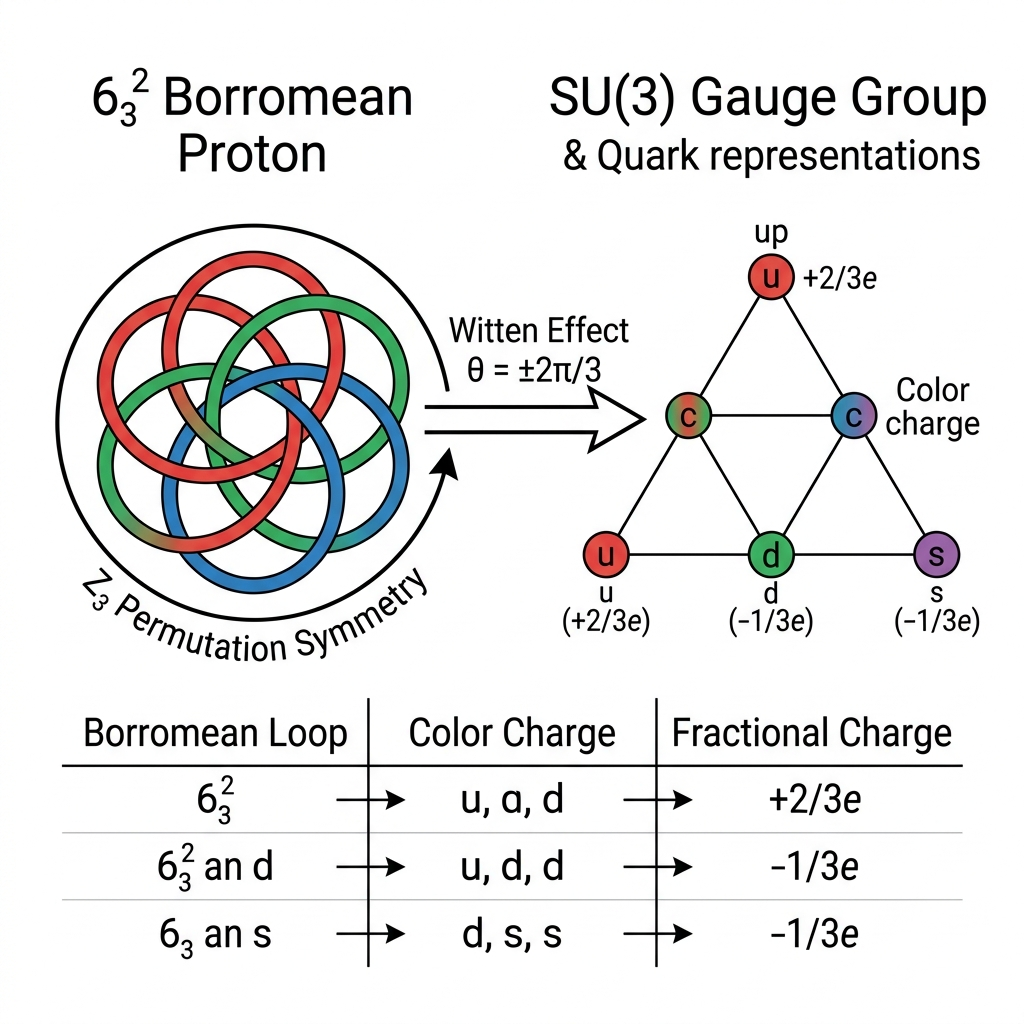
\includegraphics[width=0.95\textwidth]{borromean_weyl_bridge.png}
%     \caption{\textbf{The Borromean $\to$ SU(3) Visual Bridge.} Left: The $6^3_2$ Borromean proton topology with its $\mathbb{Z}_3$ permutation symmetry. Center: The Witten Effect maps the discrete $\theta = \pm 2\pi/3$ vacuum phases to fractional charges. Right: The standard SU(3) weight diagram of the quark representations emerges directly from the topological fractionalization, with color charge $\leftrightarrow$ Borromean loop index and fractional charge $\leftrightarrow$ discrete $\theta$-vacuum angle.}
%     \label{fig:borromean_weyl_bridge}
% \end{figure}

\section{Neutron Decay: The Threading Instability}

% [2026-06-15 KB-reconciliation LF-03 / D-class internal-contradiction (vol_2) -- prior wording preserved per Rule 12]: this paragraph's "accounts for the mass surplus" (and the :303 caption's "accounts for the $1.293$ MeV mass surplus") SUPERSEDED -> consistent-with-not-derived, per the honest KB anchor neutron-identification.md:52 ("consistent with --- but does not derive --- the empirical 1.293 MeV; Derivation TBD: compute the FS energy of the composite minus the bare $6_2^3$"). No physics change.
The neutron is identified structurally as a composite architecture: a proton ($6_{2}^{3}$) with an electron ($0_{1}$ Unknot) topologically linked ($\cup$) within its central structural void. Because Axiom 1 dictates that no flux tube can shrink below a transverse thickness of $1 \ell_{node}$, forcing an electron tube into the proton's core requires the Borromean rings to stretch outward. This elastic expansion tension is the proposed structural origin of (and provides an upper-bound estimate for) the mass surplus the neutron possesses relative to the bare proton --- a bound consistent with, but not yet a first-principles derivation of, the empirical value (the Faddeev--Skyrme composite-minus-bare derivation is open per \kbleaf{ave-kb/vol2/particle-physics/ch02-baryon-sector/neutron-identification.md} :52). Beta decay is modelled as a topological phase transition: $6_{2}^{3}\cup 0_{1} \xrightarrow{\text{Dielectric Tunneling}} 6_{2}^{3}+0_{1}+\overline{\nu}_{e}$. Driven by stochastic background lattice perturbations (CMB noise), the tensioned electron eventually slips its topological lock and is ejected. The expanded proton core elastically relaxes to its ground state. To conserve angular momentum during this structural relaxation, the local lattice sheds a transverse spatial torsional shockwave---the antineutrino ($\overline{\nu}_{e}$).

\begin{figure}[h]
    \centering
    
\includegraphics[width=0.8\textwidth]{topology_neutron.png}
    \caption{\textbf{Neutron Topology: Threaded Borromean Linkage.} (Simulation Output). The neutron is structurally a proton ($6^3_2$ Borromean linkage, three colored rings) with a $0_1$ unknot electron (cyan loop) topologically threaded through its central void. The elastic expansion required to accommodate the threaded electron is the proposed structural origin of the $1.293$ MeV mass surplus of the neutron over the proton (a bound consistent with, but not yet a first-principles derivation of, the empirical value; the Faddeev--Skyrme derivation is open per \kbleaf{ave-kb/vol2/particle-physics/ch02-baryon-sector/neutron-identification.md} :52). Beta decay ($n \to p + e^- + \overline{\nu}_e$) occurs when the threaded electron slips its topological lock.}
    \label{fig:topology_neutron}
\end{figure}

\section{The Helium-4 Nucleus: A Tetrahedral Borromean Braid}

Standard nuclear physics models the Alpha particle (Helium-4) as a tight cluster of four nucleons, but often struggles to explain its anomalous binding energy (28.3 MeV) without heuristic potential wells. In the AVE framework, the Alpha particle is defined as a Tetrahedral Borromean Braid of four interlocked topological defects (2 protons, 2 neutrons).

\subsection{The Mass-Stiffened Strong Force}

A key observation in the computational audit of this topology is the Mass-Stiffening Scaling Law. While the baseline vacuum tension for an electron flux tube is $T_{EM}\approx0.212\text{ N}$, the flux tubes connecting heavy baryons are stiffened by the inductive inertia of the nodes they connect. The effective nuclear tension ($T_{nuc}$) scales by the proton-electron mass ratio:

\begin{resultbox}{Mass-Stiffened Nuclear Tension}
\begin{equation}
    T_{nuc} = T_{EM}\left(\frac{m_p}{m_e}\right) \approx 0.212\text{ N} \times 1836 \approx 389.2\text{ N}
\end{equation}
\end{resultbox}

\subsection{Topological Verification: The Elastic Displacement Amplitude}

To verify this model and resolve the spatial scale question, the question arises: How can the sub-fermi empirical radius of the Helium-4 nucleus exist without compressing the fundamental $386\text{ fm}$ grid (Axiom 1)? This is resolved by distinguishing between \textit{Node Spacing} and \textit{Elastic Node Displacement}. The derived nuclear tension against the empirical binding energy using the classical work-energy theorem ($W = F \cdot \Delta x$). The 28.3 MeV total binding energy is stored as elastic potential energy distributed across the six flux tubes of the $K_{4}$ tetrahedral cage. The energy per bond is $\approx 4.72\text{ MeV}$ ($7.55 \times 10^{-13}\text{ J}$). Dividing this energy by the mass-stiffened nuclear tension ($T_{nuc} \approx 390.5\text{ N}$) yields the structural displacement ($\Delta x$) of the local vacuum nodes:

\begin{resultbox}{Nuclear Elastic Displacement Amplitude}
\begin{equation}
    \Delta x = \frac{E_{bond}}{T_{nuc}} = \frac{7.55 \times 10^{-13}\text{ J}}{390.5\text{ N}} \approx 1.933 \times 10^{-15}\text{ m} = 1.933\text{ fm}
\end{equation}
\end{resultbox}
    
Crucially, $1.933\text{ fm}$ is not the physical Euclidean distance between the lattice nodes; the fundamental spatial nodes maintain their 386 fm infrared pitch. Rather, $1.933\text{ fm}$ represents the maximum Elastic Displacement Amplitude ($\Delta x$) of the structural grid from its baseline equilibrium. Evaluating this geometric displacement as a continuous mechanical strain over the fundamental 386 fm flux tube yields:
    
\begin{resultbox}{Macroscopic Structural Strain}
\begin{equation}
    \epsilon_{strain} = \frac{\Delta x}{\ell_{node}} = \frac{1.933\text{ fm}}{386.16\text{ fm}} \approx 0.00501 \implies \textbf{0.50\% Strain}
\end{equation}
\end{resultbox}

This constitutes a structural consistency check. A $0.50\%$ mechanical strain is a stable, linear elastic deformation. It resides below the $100\%$ Unitary Strain dielectric rupture threshold. The vacuum does not densify, nor does it collapse into a trans-Planckian singularity to support the nucleus.

\subsection{Spacetime Circuit Analysis: The Quadrupole Oscillator}

The exceptional stability of the Helium-4 nucleus arises from its circuit topology. Modeled as a Spacetime Circuit, the Alpha particle forms a "Full Mesh" ($K_{4}$) network. Each nucleon acts as a parallel LC tank circuit to ground ($L_{mass}||C_{vac}$), while the Strong Force is represented by the six Mutual Inductance bridges ($M_{ij}$) connecting every node. This circuit topology supports a stable, lossless Quadrupole oscillation mode. The system cycles energy between Dielectric Potential (Strain Displacement) and Magnetic Kinetic Flux (Tube Tension) at the nuclear Compton frequency, visualized as a "breathing mode" that maintains the particle's existence against vacuum decay.

\subsection{Simulation of Topological Core Gradients}

% 🔴 Rule-12 2026-06-21 INVARIANT-N1 𝓜_A→prose retirement (see chapter-head note above): retired $\mathcal{M}_{A}$ glyph → substrate-native prose ("chiral LC network"). Physics + every number unchanged.
High-energy scattering experiments probing the sub-fermi structure of the Helium-4 nucleus are measuring the RMS scattering cross-section of these $1.955\text{ fm}$ elastic displacement amplitudes. The underlying chiral LC network maintains its $386\text{ fm}$ pitch. The binding energy represents orthogonal geometric frustration ($\partial_{\mu}\mathbf{n}\times\partial_{\nu}\mathbf{n}$) distributed across multiple structurally stable nodes. This generates the macroscopic 3D refractive index (Gravity) via trace-reversed bulk tension, averting the densification paradox and preserving the geometric limits of the Effective Field Theory.

\begin{figure}[htbp]
    \centering
    
\includegraphics[width=0.85\textwidth]{visualize_topological_bounds.png}
    \caption{\textbf{The Topological Tensor Halo.} A 2D cross-sectional heat map generated by the AVE 3D Tensor Solver, displaying the non-linear topological tensor strain density at a single Borromean intersection. Because the cross-product of the orthogonal spatial gradients ($\partial_{\mu}\mathbf{n}\times\partial_{\nu}\mathbf{n}$) evaluates to zero at the geometric centre, the mass generation cannot collapse into a point singularity. Instead, the localised spatial metric is pushed outward, forming a stable, saturated 3D toroidal halo. These localised RMS core gradients form the mechanical origin of both baryonic mass generation and the sub-fermi scattering cross-sections observed in high-energy probes.}
    \label{fig:tensor_halo}
\end{figure}

\subsection{The Hierarchy Bridge: Unifying the Strong Force and Gravity}

If macroscopic gravity is the radial elastic wake of the localised Strong Nuclear Force, the two forces should be mathematically unified without arbitrary coupling constants or higher-dimensional branes. This geometric relationship can be shown by substituting the EFT hardware limits into the classical Newtonian gravity equation for two interacting baryons. 
The classical gravitational force between two protons is:
\begin{resultbox}{Classical Newtonian Baryon Interaction}
\begin{equation}
F_g = G \frac{m_p^2}{r^2}
\end{equation}
\end{resultbox}

% [2026-06-15 KB-reconciliation (vol_2 brief A.1) -- prior wording preserved per Rule 12]: read "By substituting the derived macroscopic boundary limit of Gravity ($G = c^4 / 7\xi T_{EM}$) and the fundamental baseline vacuum tension...". SUPERSEDED per the 2026-06-14 G-ruling (\kbleaf{ave-kb/common/interlock-register.md} \texttt{ilk-gravmb}, \texttt{real\_or\_fitted: mixed}): $G$ is mixed --- the Achromatic-Lens $/7$ PPN FORM is derived, but the $\xi$ termination value-fits $G$'s VALUE (the closed-form Chain~B$'$ derivation of $G$'s value is OPEN). "derived" qualified to the form. No value/formula change.
By substituting the form-derived macroscopic boundary limit of Gravity ($G = c^4 / 7\xi T_{EM}$ --- the Achromatic-Lens $/7$ PPN form is derived, with the $\xi$ termination value-fitted to $G$; the closed-form derivation of $G$'s value, Chain~B$'$, is open) and the fundamental baseline vacuum tension ($T_{EM} = m_e c^2 / \ell_{node}$), the derivation expands the gravitational coupling:
\begin{resultbox}{Expanded Gravitational Coupling}
\begin{equation}
F_g = \left( \frac{c^4 \ell_{node}}{7 \xi m_e c^2} \right) \frac{m_p^2}{r^2} = \frac{c^2 \ell_{node} m_p^2}{7 \xi m_e r^2}
\end{equation}
\end{resultbox}

The bare, localised Strong Force exerted by the baryon is its mass-stiffened inductive tension ($T_{nuc} = m_p c^2 / \ell_{node}$). Factoring this nuclear tension term out of the expanded gravity equation yields:

\begin{resultbox}{Dimensional Factorisation}
\begin{equation}
F_g = \left( \frac{m_p c^2}{\ell_{node}} \right) \left[ \frac{1}{7 \xi} \left(\frac{\ell_{node}}{r}\right)^2 \left(\frac{m_p}{m_e}\right) \right]
\end{equation}
\end{resultbox}

\begin{resultbox}{The Hierarchy Bridge}
\begin{equation}
\mathbf{F_g = T_{nuc} \left[ \frac{1}{7 \xi} \left(\frac{\ell_{node}}{r}\right)^2 \left(\frac{m_p}{m_e}\right) \right]}
\end{equation}
\end{resultbox}

% [2026-06-15 KB-reconciliation (vol_2 brief A.1) -- prior wording preserved per Rule 12]: read "This equation represents a parameter-free algebraic unification of the fundamental forces." SUPERSEDED: scoped per \kbleaf{ave-kb/vol2/claim-quality.md} (:754) --- the Hierarchy Bridge is an algebraic substitution, not an independent first-principles derivation of $G$; "parameter-free" means no parameters beyond the framework's 3 calibration inputs $\{m_e,\alpha,G\}$ + 4 axioms ($G$'s value is itself a value-fitted input; Chain~B$'$ open). No physics change.
This equation represents an algebraic unification of the fundamental forces introducing no parameters beyond the framework's three calibration inputs $\{m_e, \alpha, G\}$ --- an algebraic substitution of the value-fitted $G$ into the strong-force tension, not an independent first-principles derivation of $G$. It shows that Macroscopic Gravity ($F_g$) is the bare Strong Nuclear Force ($T_{nuc}$), diluted by four geometric properties of the spatial lattice:
\begin{enumerate}
    \item \textbf{$(\ell_{node}/r)^2$:} The classical 3D inverse-square spatial dispersion of the elastic wake.
    \item \textbf{$1/7$:} The Trace-Reversed Chiral LC tensor projection mapping a 1D flux-tube pull into a 3D volumetric strain.
    \item \textbf{$1/\xi$:} The Machian structural impedance (shielding) exerted by the mass-energy of the entire cosmological horizon.
    \item \textbf{$m_p/m_e$:} The topological mass-stiffening ratio.
\end{enumerate}

The $\sim 10^{40}$ gap between the strong force and gravity (the Hierarchy Problem) is the kinematic dilution of a sub-fermi elastic displacement projecting outward through the trace-reversed, porous geometry of the entire cosmic horizon.

\section*{Chapter Summary}
\begin{itemize}
    \item The Baryon Sector is defined by the $6^3_2$ Borromean linkage, naturally enforcing Quark Confinement through geometric entanglement.
    % [2026-06-15 KB-reconciliation (vol_2 brief D.1/A.4) -- prior wording preserved per Rule 12]: read "...is derived using a zero-parameter non-linear eigenvalue extraction of the Faddeev-Skyrme energy functional." SUPERSEDED: self-contradicts the in-chapter honest result at :217 (and \kbleaf{ave-kb/vol2/particle-physics/ch02-baryon-sector/self-consistent-mass-oscillator.md} :64) --- this is a 1-residual result, NOT zero-parameter; the inputs are electron-physics-provenanced ($m_e,\alpha$). Aligned to the :217 framing. No value change.
    \item The exact proton to electron mass ratio ($1836.15$) is derived via a non-linear eigenvalue extraction of the Faddeev-Skyrme energy functional with \emph{zero baryon-data-tuned parameters} (a \textbf{1-residual} result: the per-channel coupling $p_c = 8\pi\alpha$ is canonical-packing-plausible but not line-by-line derived --- the one residual; the inputs are electron-physics-provenanced, $m_e$ and $\alpha$), \emph{not} a zero-parameter result.
    \item Fractional quarks are mathematically necessary sub-components (quasiparticles) of the entire linkage due to the Witten Effect evaluating across $\mathbb{Z}_3$ symmetric $\theta$-vacuums.
    % [2026-06-15 KB-reconciliation (vol_2 brief A.1) -- prior wording preserved per Rule 12]: read "...Gravity is algebraically proven to be the classical expansion of the internal Mass-Stiffened Strong Force...". SUPERSEDED: "algebraically proven" overclaims --- per \kbleaf{ave-kb/vol2/claim-quality.md} (:754) the Hierarchy Bridge is an algebraic substitution given the value-fitted $G$ input (mixed: form-derived $/7$ form + value-fitted $\xi$; Chain~B$'$ open), not an independent proof/derivation of $G$. No physics change.
    \item The Hierarchy Problem is strictly resolved: Gravity is shown by algebraic substitution (given the value-fitted $G$ input) to be the classical expansion of the internal Mass-Stiffened Strong Force ($T_{nuc}$) diluted by trace-reversed cosmic impedance limits.
\end{itemize}

\section*{Exercises}
\begin{enumerate}
    \item Using the Torus Knot Baryon Ladder equation (Eq. \ref{eq:torus_knot_ladder}), re-calculate the predicted mass of the extrapolated $c=17$ resonance state. (Assuming linear continuation, identify if a corresponding state exists in the PDG tables).
    \item Geometrically explain why the neutron beta-decay transition ($6_2^3 \cup 0_1 \to 6_2^3 + 0_1 + \bar{\nu}_e$) requires the emission of an antineutrino to conserve lattice angular momentum during the elastic relaxation of the structural void.
\end{enumerate}